%%%%%%%%%%%%%%%%%%%%%%%%%%%%%%%%%%%%%%%%%
% Short Sectioned Assignment LaTeX Template Version 1.0 (5/5/12)
% This template has been downloaded from: http://www.LaTeXTemplates.com
% Original author:  Frits Wenneker (http://www.howtotex.com)
% License: CC BY-NC-SA 3.0 (http://creativecommons.org/licenses/by-nc-sa/3.0/)
%%%%%%%%%%%%%%%%%%%%%%%%%%%%%%%%%%%%%%%%%

%----------------------------------------------------------------------------------------
%	PACKAGES AND OTHER DOCUMENT CONFIGURATIONS
%----------------------------------------------------------------------------------------

\documentclass[paper=a4, fontsize=11pt]{scrartcl} % A4 paper and 11pt font size

% ---- Entrada y salida de texto -----

\usepackage[T1]{fontenc} % Use 8-bit encoding that has 256 glyphs
\usepackage[utf8]{inputenc}
%\usepackage{fourier} % Use the Adobe Utopia font for the document - comment this line to return to the LaTeX default

% ---- Idioma --------

\usepackage[spanish, es-tabla]{babel} % Selecciona el español para palabras introducidas automáticamente, p.ej. "septiembre" en la fecha y especifica que se use la palabra Tabla en vez de Cuadro

\usepackage{eurosym}
\usepackage{enumitem}

% ---- Otros paquetes ----

\usepackage{url} % ,href} %para incluir URLs e hipervínculos dentro del texto (aunque hay que instalar href)
\usepackage{amsmath,amsfonts,amsthm} % Math packages
%\usepackage{graphics,graphicx, floatrow} %para incluir imágenes y notas en las imágenes
\usepackage{graphics,graphicx, float} %para incluir imágenes y colocarlas

% Para hacer tablas comlejas
%\usepackage{multirow}
%\usepackage{threeparttable}

%\usepackage{sectsty} % Allows customizing section commands
%\allsectionsfont{\centering \normalfont\scshape} % Make all sections centered, the default font and small caps

\usepackage{fancyhdr} % Custom headers and footers
\pagestyle{fancyplain} % Makes all pages in the document conform to the custom headers and footers
\fancyhead{} % No page header - if you want one, create it in the same way as the footers below
\fancyfoot[L]{} % Empty left footer
\fancyfoot[C]{} % Empty center footer
\fancyfoot[R]{\thepage} % Page numbering for right footer
\renewcommand{\headrulewidth}{0pt} % Remove header underlines
\renewcommand{\footrulewidth}{0pt} % Remove footer underlines
\setlength{\headheight}{13.6pt} % Customize the height of the header

\numberwithin{equation}{section} % Number equations within sections (i.e. 1.1, 1.2, 2.1, 2.2 instead of 1, 2, 3, 4)
\numberwithin{figure}{section} % Number figures within sections (i.e. 1.1, 1.2, 2.1, 2.2 instead of 1, 2, 3, 4)
\numberwithin{table}{section} % Number tables within sections (i.e. 1.1, 1.2, 2.1, 2.2 instead of 1, 2, 3, 4)

\setlength\parindent{0pt} % Removes all indentation from paragraphs - comment this line for an assignment with lots of text

\newcommand{\horrule}[1]{\rule{\linewidth}{#1}} % Create horizontal rule command with 1 argument of height


%----------------------------------------------------------------------------------------
%	TÍTULO Y DATOS DEL ALUMNO
%----------------------------------------------------------------------------------------

\title{	
\normalfont \normalsize 
\textsc{\textbf{Ingeniería de Servidores (2016-2017)} \\ Grado en Ingeniería Informática \\ Universidad de Granada} \\ [25pt] % Your university, school and/or department name(s)
\horrule{0.5pt} \\[0.4cm] % Thin top horizontal rule
\huge Memoria Práctica 2 \\ % The assignment title
\horrule{2pt} \\[0.5cm] % Thick bottom horizontal rule
}

\author{Cristian Vélez Ruiz} % Nombre y apellidos

\date{\normalsize\today} % Incluye la fecha actual

%----------------------------------------------------------------------------------------
% DOCUMENTO
%----------------------------------------------------------------------------------------
\begin{document}

\maketitle % Muestra el Título

\newpage %inserta un salto de página

\tableofcontents % para generar el índice de contenidos

\listoffigures

\listoftables

\newpage

%----------------------------------------------------------------------------------------
%	Cuestión 1
%----------------------------------------------------------------------------------------
\section[Cuestión 1]{a) Liste los argumentos de yum necesarios para instalar,buscar y eliminar paquetes. b)¿Qué ha de hacer para que yum pueda tener acceso a Internet en el PC del aula?(Pistas: archivo de configuración en /etc,proxy: stargate.ugr.es:3128)c)¿Cómo añadimos un nuevo repositorio?}



\begin{enumerate}[label=(\alph*)]
	\item  \textbf{Instalar: } \textit{sudo yum install programa}\\
	\textbf{Eliminar: } \textit{sudo yum remove programa}\\
	\textbf{Buscar: } \textit{yum search programa}
	
	\item Para poder acceder a través del ordenador de el aula necesitamos añadir en el fichero /etc/yum.conf en la última linea proxy=stargate.ugr.es:3128.
	
	\item Para añadir un repositorio usamos sudo \textit{yum-config-manager --add-repo=repositorio} \cite{yum}
\end{enumerate}

%------------------------------------------------

%----------------------------------------------------------------------------------------
%	Cuestión 2
%----------------------------------------------------------------------------------------
\section[Cuestión 2]{a)Liste los argumentos de apt necesarios para instalar, buscar y eliminar paquetes.b)¿Qué ha de hacer para que apt pueda tener acceso a Internet en el PC del aula?(Pistas: archivo de configuración en /etc, proxy: stargate.ugr.es:3128)c)¿Cómo añadimos un nuevo repositorio?}

\begin{enumerate}[label=(\alph*)]
	\item  \textbf{Instalar: } \textit{sudo apt-get install programa}\\
	\textbf{Eliminar: } \textit{sudo apt-get remove programa}\\
	\textbf{Buscar: } \textit{apt-cache search programa}
	
	\item Si existe el archivo /etc/apt/apt.conf solo tendremos que añadir en la ultima linea \textit{Acquire::http::Proxy "http://stargate.ugr.es:3128";}, en el caso de que no existiese ese archivo lo crearíamos y añadiríamos esa linea. \cite{apt}
	
	\item Para añadir un nuevo repositorio \textit{sudo add-apt-repository repositorio}\cite{apt}

\end{enumerate}
%----------------------------------------------------------------------------------------
%	Cuestión 3
%----------------------------------------------------------------------------------------
\section[Cuestión 3]{a)¿Con qué comando puede abrir/cerrar un puerto usando ufw? Muestre un ejemplo de cómo lo ha hecho	b)¿Con qué comando puede abrir/cerrar un puerto usando firewall-cmd en CentOS? Muestre un ejemplo de cómo lo ha hecho c)Utilice el comando nmap para ver que,efectivamente, los puertos están accesibles}

Nmap no detecta los puertos si no existe un servicio detrás de cada uno escuchando, por ello mostrare el estado del firewall.

\begin{enumerate}[label=(\alph*)]
	\item En mi caso lo que voy a hacer primero es cerrar el puerto 80, para ello lo que haré es \textit{sudo ufw deny 80}, a continuación se puede ver que se deniegan tanto para IPv4 y IPv6, el uso del puerto 80.Después para dejarlo todo como estaba lo que voy a hacer es permitir otra vez el uso del puerto 80 con \textit{sudo ufw allow 80} y mostrar el estado del firewall.
	(Con el uso de NMAP no detectaba cambios)
	
		\begin{figure}[H]
		\centering
		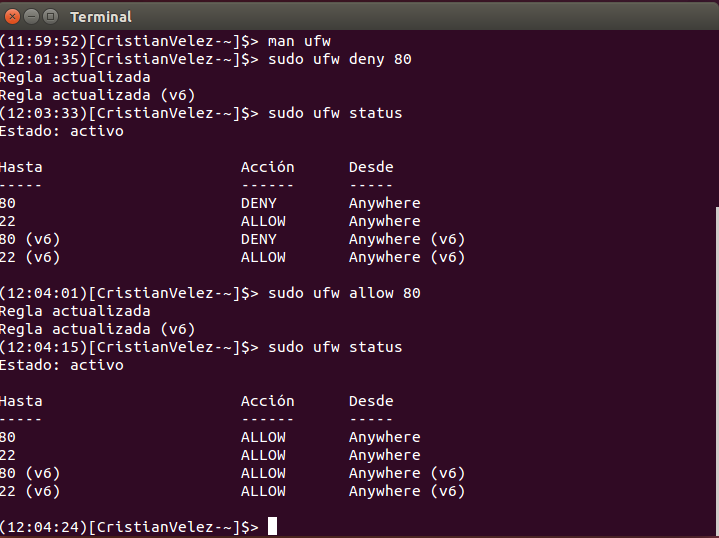
\includegraphics[scale=0.5]{pics/1_ufw.png}  
		\caption{Ufw allow y deny} \label{fig:figura11}
	\end{figure}

	\item En el caso de centOS lo que vamos a hacer es permitir el uso de ftp, para ello vamos a hacer firewall-cmd --add-service=ftp --permanent, después vamos a reiniciar el firewall con firewall-cmd --reload, mostraré el estado antes y después de este proceso.
	
			\begin{figure}[H]
		\centering
		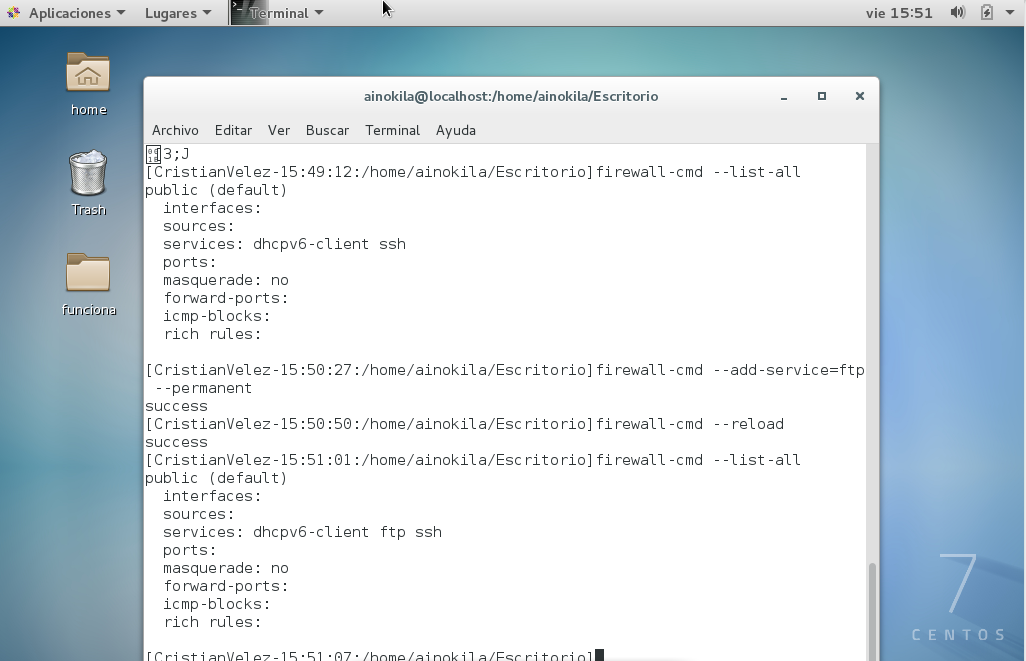
\includegraphics[scale=0.5]{pics/ufwadd.png}  
		\caption{Firewall-cmd permitiendo servicio} \label{fig:fwcmdadd}
		\end{figure}
	
	Para revertir el proceso, vamos a eliminar el uso del servicio, firewall-cmd --remove-service=ftp --permanent y después reiniciamos el firewall.
	
	\begin{figure}[H]
		\centering
		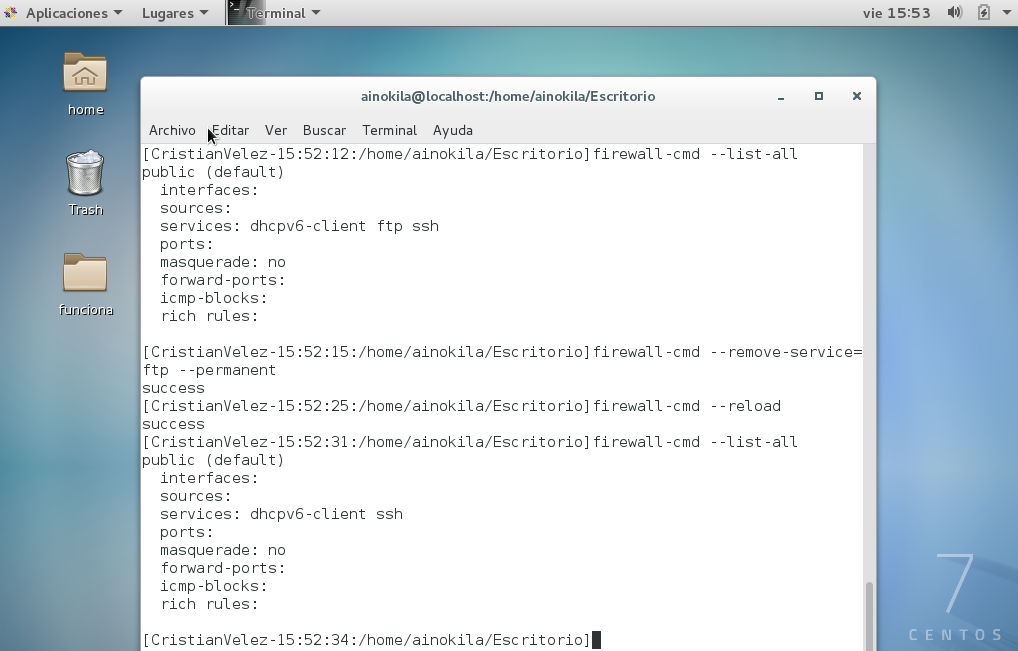
\includegraphics[scale=0.5]{pics/ufwremo.png}  
		\caption{Firewall-cmd denegando servicio} \label{fig:fwcmdadd}
	\end{figure}

	También si quisiéramos añadir un puerto específico valdría con  \textit{firewall-cmd --add-port=8888 --permanent}, después reiniciar el firewall con \textit{firewall-cmd --reload}, y para eliminarlo sería con \textit{firewall-cmd --remove-port=8888 --permanent} y \textit{firewall-cmd --reload}.
	
	\item Para usar nmap contra nosotros mismos tenemos que lanzar la orden \textit{nmap localhost}, nos analizará los puertos que estén abiertos y que tengan un servicio detrás escuchando, si eso no ocurre nmap no podrá detectar el puerto.
	
	
	
	
	
\end{enumerate}

%----------------------------------------------------------------------------------------
%	Cuestión 4
%----------------------------------------------------------------------------------------
\section[Cuestión 4]{¿Qué diferencia hay entre telnet y ssh?}

Ambos se usan para conectarse mediante terminal a otro ordenador o servidor, la diferencia entre ellos y que ha determinado que Telnet apenas se use en comparación con ssh es su seguridad principalmente. En Telnet tanto la información como las contraseñas y usuarios viajan en texto plano, mientras que con ssh los datos viajan cifrados lo que nos ofrece una mayor seguridad. \cite{SSH}

%----------------------------------------------------------------------------------------
%	Cuestión 5
%----------------------------------------------------------------------------------------
\section[Cuestión 5]{a)¿Para qué sirve la opción -X? b)Ejecute remotamente, es decir, desde la máquina anfitriona (si tiene Linux) o desde la otra máquina	virtual, el comando	gedit en una sesión abierta con ssh. ¿Qué ocurre?}

\begin{enumerate}[label=(\alph*)]
	\item Cuando se usa la opción -X en ssh en una aplicación en ambos debe estar instalada, y su funcionamiento es mostrarnos a nosotros la interfaz,y mandar solo mediante ssh las llamadas del sistema o simplemente lo que se le escriba, pero nunca manda la interfaz a través de ssh lo que hace que aumente su ligereza y su funcionamiento sea mas fluido.	
	
	\item Primero lanzamos el comando \textit{ssh -X 10.0.2.6}, añadimos la contraseña y conectara, ahora lanzaremos gedit ./pruebaSsh 
	
	\begin{figure}[H]
		\centering
		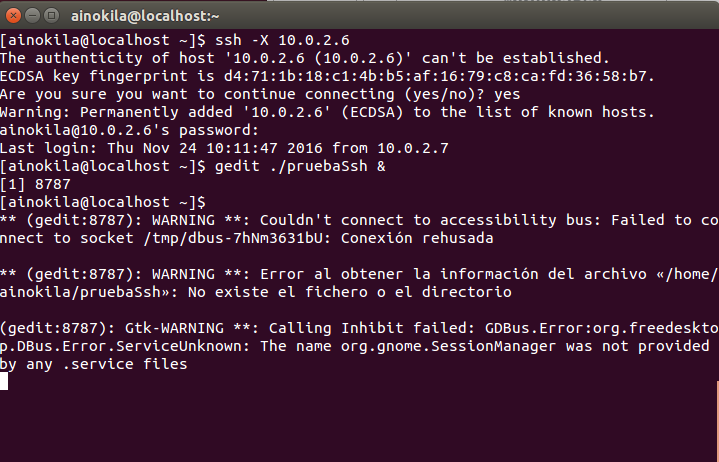
\includegraphics[scale=0.35]{pics/ssh_1.png}  
		\caption{ssh -X paso 1} \label{fig:ssh_1}
	\end{figure}

	Una vez se nos abra gedit escribimos el texto y guardamos.

	\begin{figure}[H]
		\centering
		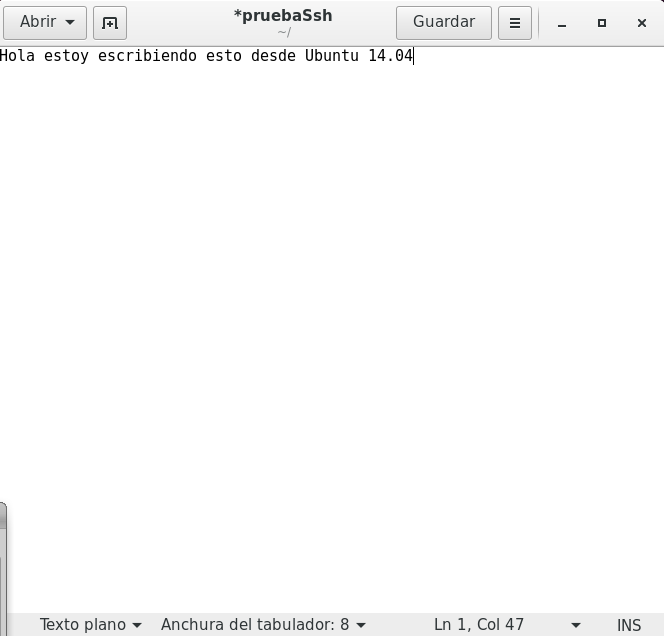
\includegraphics[scale=0.35]{pics/shh_2.png}  
		\caption{ssh -X paso 2} \label{fig:ssh_2}
	\end{figure}

	Como vemos se nos ha guardado una archivo en CentOS.
	\begin{figure}[H]
	\centering
	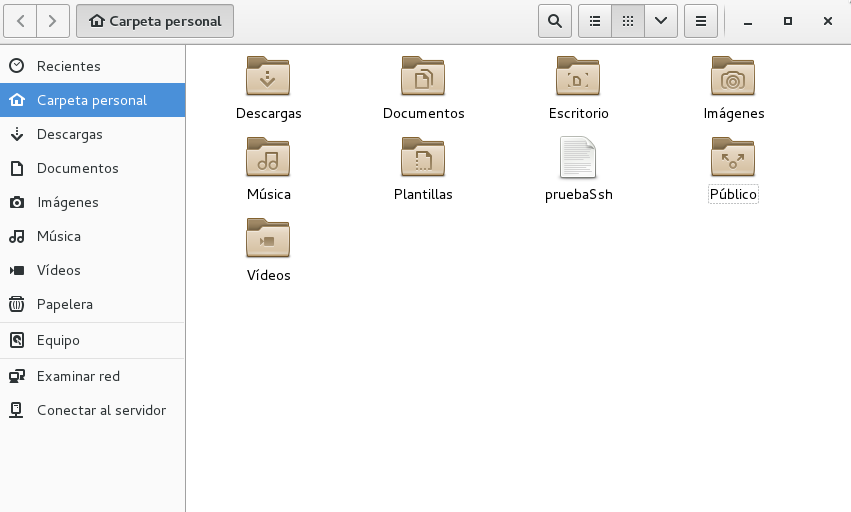
\includegraphics[scale=0.35]{pics/ssh_3.png}  
	\caption{ssh -X paso 3} \label{fig:ssh_3}
	\end{figure}

	Tenemos la información que escribimos desde Ubuntu.
	\begin{figure}[H]
		\centering
		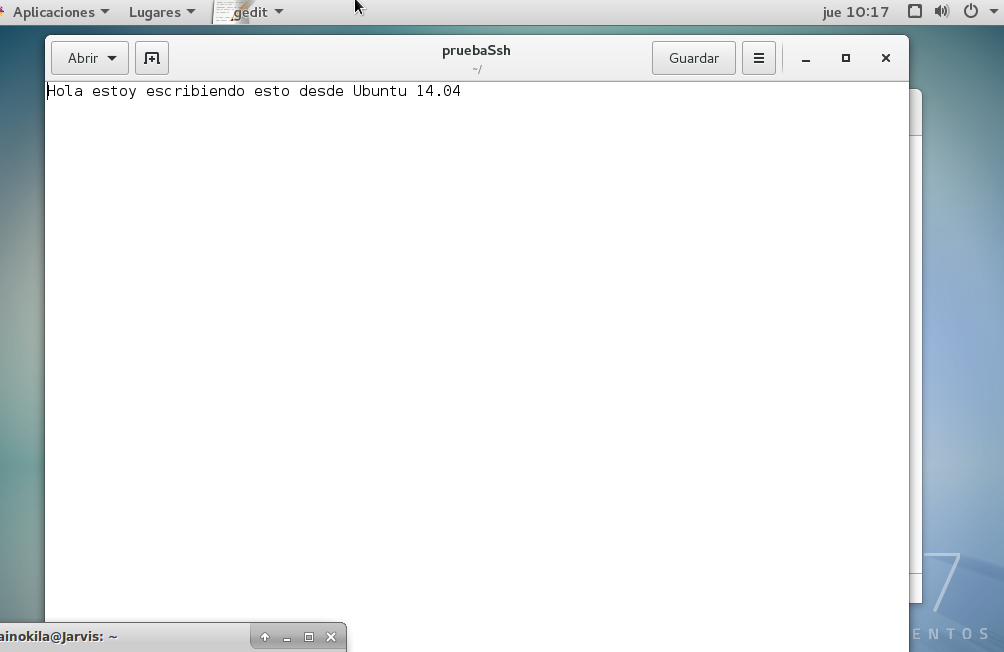
\includegraphics[scale=0.35]{pics/ssh_4.png}  
		\caption{ssh -X paso 4} \label{fig:ssh_4}
	\end{figure}

	
	
\end{enumerate}

%----------------------------------------------------------------------------------------
%	Cuestión 6
%----------------------------------------------------------------------------------------
\section[Cuestión 6]{ Muestre la secuencia de comandos y las modificaciones a los	archivos correspondientes para permitir acceder a la consola remota sin introducir la contraseña. Pruebe que funciona. (Pistas: ssh-keygen, ssh-copy-id).}

Primero lo que tenemos es generar un par de claves para la conexión, lo que haremos es \textit{ssh-keygen -b 4096 -t rsa} , introducimos la contraseña para tener bien guardadas las claves.

	\begin{figure}[H]
	\centering
	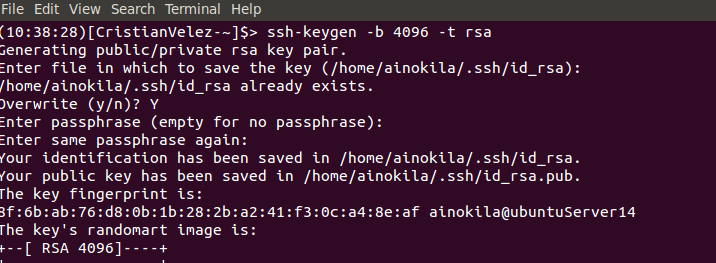
\includegraphics[scale=0.35]{pics/ssh_gen.png}  
	\caption{Ssh-keygen} \label{fig:ssh_keygen}
	\end{figure}

Una vez que tenemos nuestras claves, procedemos a 'dar' la clave, para que se puedan conectar a nosotros,introducimos \textit{ssh-copy-id ainokila@10.0.2.7} , con esto estamos copiando la clave para poder acceder,aquí nos pedirá que desbloqueemos las claves.

	\begin{figure}[H]
	\centering
	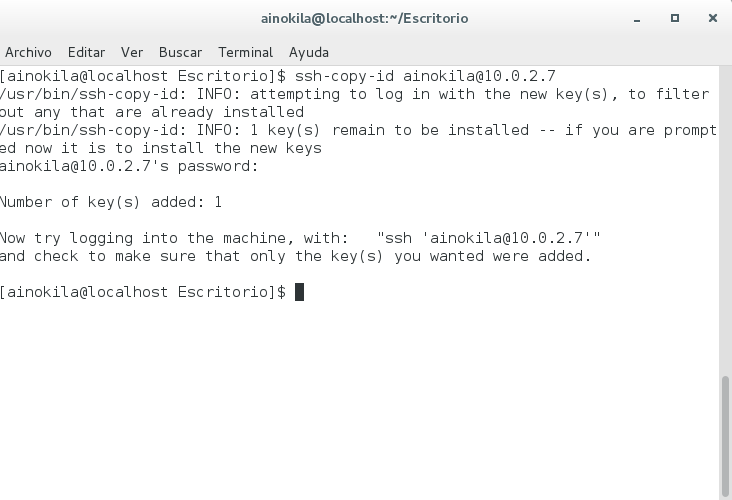
\includegraphics[scale=0.35]{pics/ssh_copy.png}  
	\caption{Ssh-copy-id} \label{fig:ssh_copy}
\end{figure}

Ahora finalmente ya podemos conectarnos sin estar repitiendo una y otra vez la contraseña. \cite{key}

	\begin{figure}[H]
	\centering
	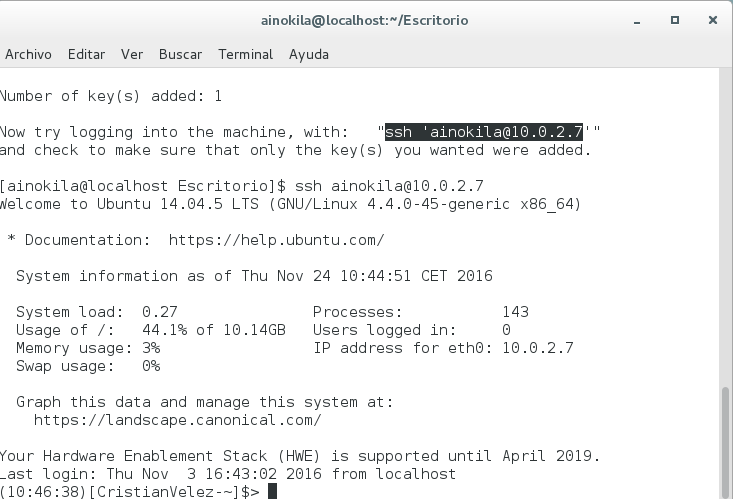
\includegraphics[scale=0.35]{pics/ssh_conect.png}  
	\caption{Ssh sin contraseña conexión} \label{fig:ssh_conect}
\end{figure}



%----------------------------------------------------------------------------------------
%	Cuestión 7
%----------------------------------------------------------------------------------------
\section[Cuestión 7]{ ¿Qué archivo es el que contiene la configuración del servicio ssh? ¿Qué parámetro hay que modificar para evitar que el usuario root acceda? Cambie el puerto por defecto y compruebe que puede acceder.}

Las configuraciones de ssh están en el archivo de configuración del demonio de ssh \textit{/etc/ssh/sshd\_config}, para poder cambiar que el usuario root no pueda acceder, tenemos que cambiar en la linea donde pone PermitRootLogin a no, lo que impedirá que el usuario root pueda acceder.

Para cambiar el puerto de ssh vamos a ir al archivo \textit{/etc/ssh/sshd\_config} y donde pone port 22 lo cambiaremos por port 2222 para usar el puerto 2222, una vez hecho esto reiniciamos el servicio para que se apliquen los cambios con \textit{sudo service ssh restart}, ahora accederemos mendiante \textit{ssh ssh -p 2222 localhost}.\cite{key}

	\begin{figure}[H]
	\centering
	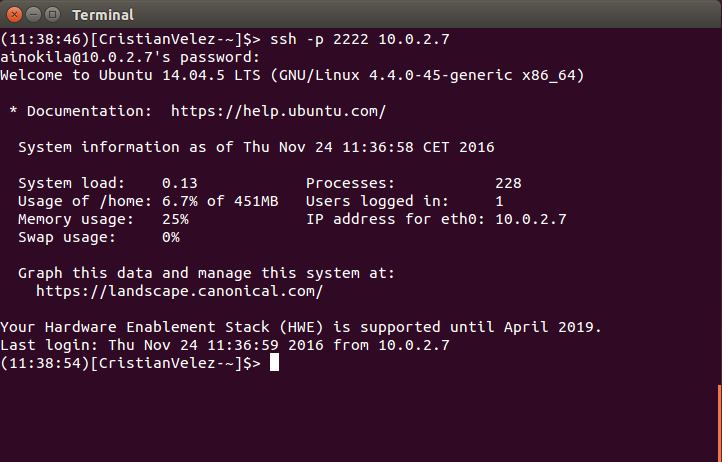
\includegraphics[scale=0.35]{pics/ssh_port_2222.png}  
	\caption{Ssh puerto 2222} \label{fig:ssh_conect}
	\end{figure}
%----------------------------------------------------------------------------------------
%	Cuestión 8
%----------------------------------------------------------------------------------------
\section[Cuestión 8]{ Indique si es necesario reiniciar el servicio ¿Cómo se reinicia	un servicio en Ubuntu? ¿y en CentOS? Muestre la secuencia de comandos para hacerlo.}

Si, ya que es necesario para que vuelva a leer el archivo de configuración que hemos editado, ya que por el contrario tendrá la configuración de cuando se lanzo el servicio por última vez.

Para Ubuntu es como hicimos en el anterior ejercicio con \textit{service servicio restart} y en CentOS  \textit{sudo systemctl enable/start servicio}.


%	Cuestión 9
%----------------------------------------------------------------------------------------
\section[Cuestión 9]{ Muestre los comandos que ha utilizado en Ubuntu Server y en	CentOS (aunque en este último puede utilizar la GUI, en tal caso, realice	capturas de pantalla). Compruebe que la instalación ha sido correcta.}

En Ubuntu tenemos que instalarlo mendiante el comando \textit{sudo apt-get install -y lamp-server\^} con esa orden nos instalara todos los paquetes necesarios.\\

	\begin{figure}[H]
	\centering
	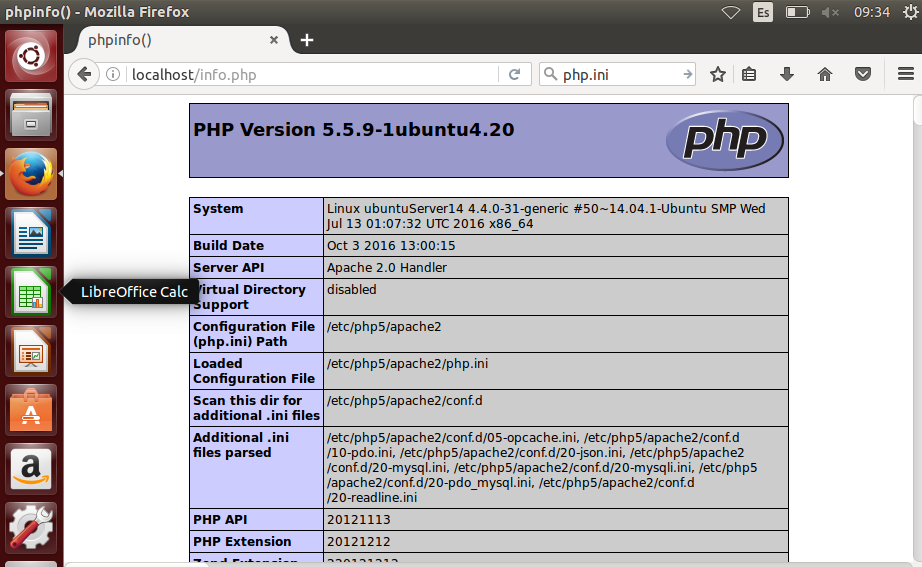
\includegraphics[scale=0.35]{pics/lamp.png}  
	\caption{Lamp Ubuntu} \label{fig:lamp}
	\end{figure}




En CentOS tenemos que ir instalándolos individualmente, \textit{sudo yum install httpd} instalamos el demonio de httpd ,después necesitamos instalar php con \textit{sudo yum install php}, y por último la base de datos mariadb con \textit{sudo yum install mariadb-server}

	\begin{figure}[H]
	\centering
	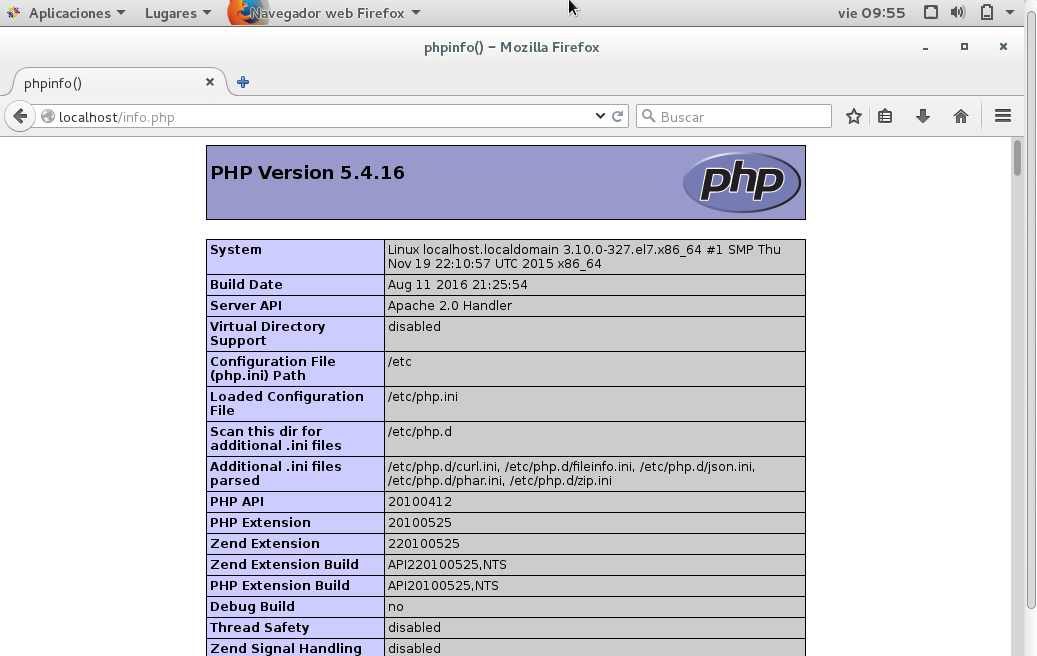
\includegraphics[scale=0.35]{pics/lamp_centos.png} 
	\caption{Lamp CentOS} \label{fig:lamp_cen}
	\end{figure}

%----------------------------------------------------------------------------------------
%	Cuestión 10
%----------------------------------------------------------------------------------------
\section[Cuestión 10]{ Realice la instalación usando GUI o PowerShell y compruebe	que el servicio está funcionando accediendo a la MV a través de la anfitriona. }

Para realizar la instalación vamos a la pantalla inicial y le damos a \textit{Add features} 

	\begin{figure}[H]
	\centering
	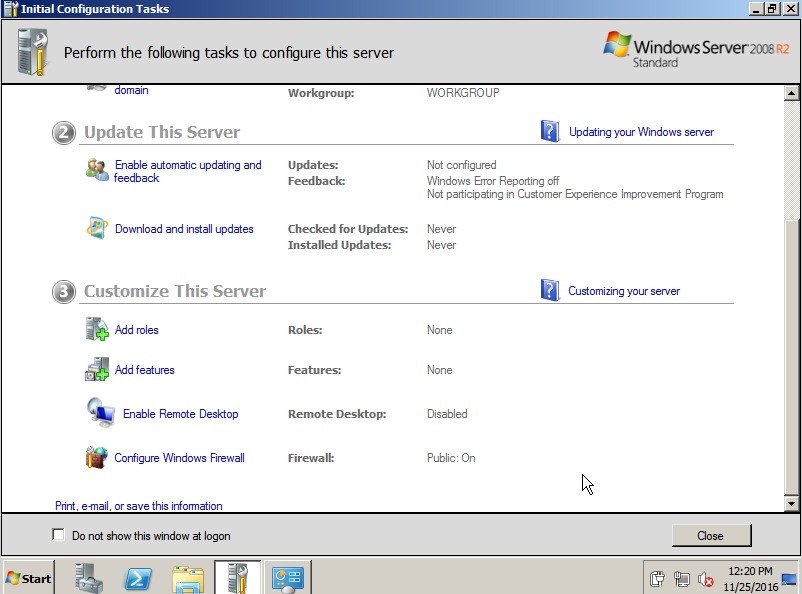
\includegraphics[scale=0.35]{pics/gui1.png} 
	\caption{ISS Paso 1} \label{fig:iss1}
	\end{figure}

A continuacion seleccionamos ISS Server Extension,y damos siguiente,

	\begin{figure}[H]
	\centering
	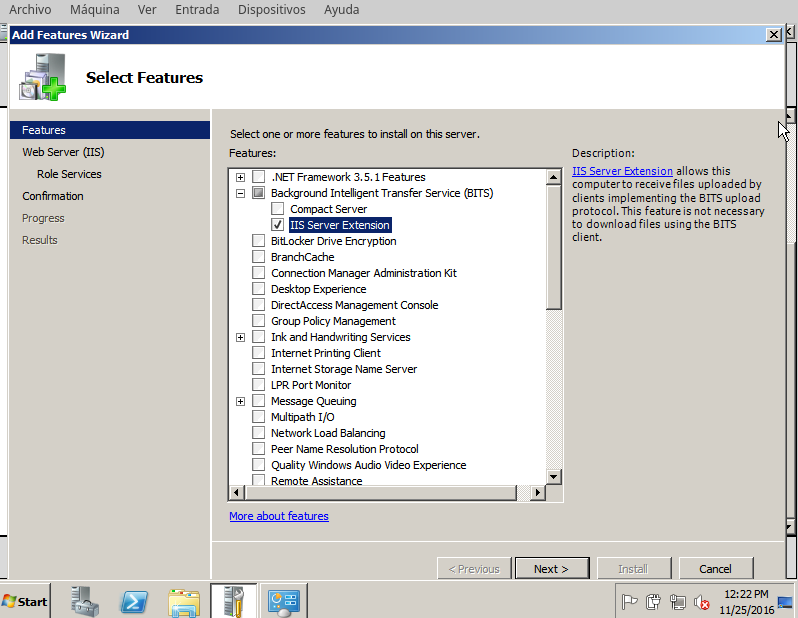
\includegraphics[scale=0.35]{pics/gui2.png} 
	\caption{ISS Paso 2} \label{fig:iss2}
	\end{figure}

Ahora seleccionamos ftp y damos otra vez next,

	\begin{figure}[H]
	\centering
	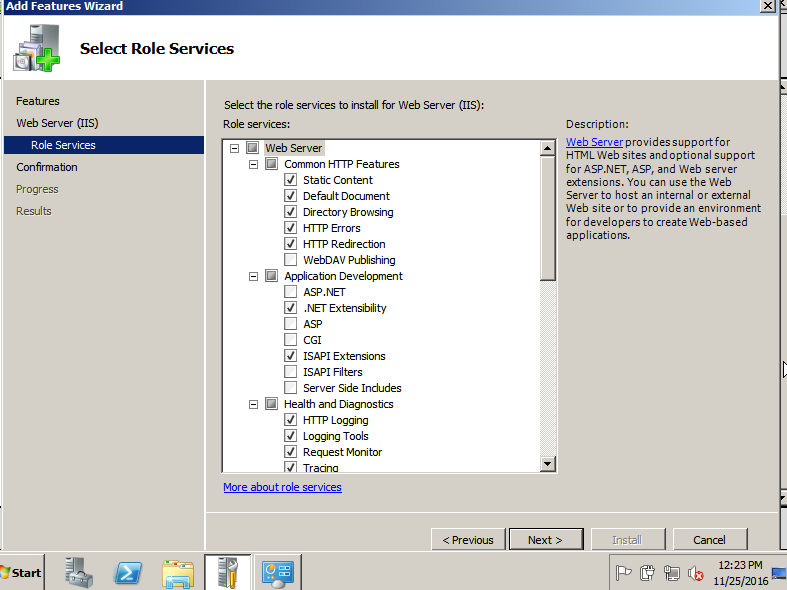
\includegraphics[scale=0.35]{pics/gui3.png} 
	\caption{ISS Paso 3} \label{fig:iss3}
	\end{figure}

Damos a install y se instalara ISS,

	\begin{figure}[H]
	\centering
	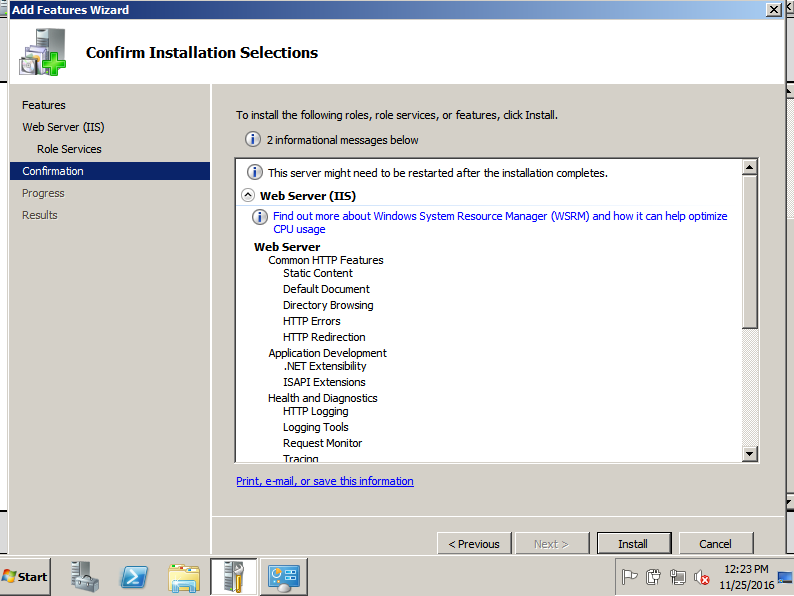
\includegraphics[scale=0.35]{pics/gui4.png} 
	\caption{ISS Paso 4} \label{fig:iss4}
	\end{figure}

Finalmente comprobamos su funcionamiento,

	\begin{figure}[H]
	\centering
	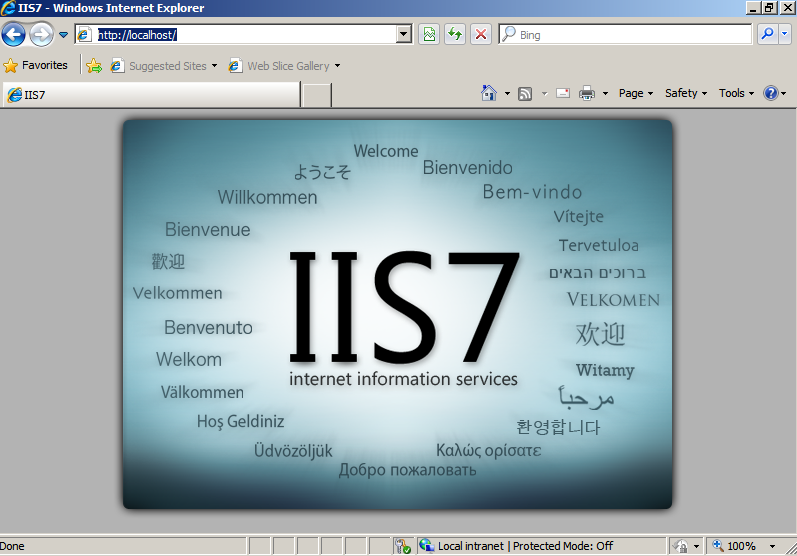
\includegraphics[scale=0.35]{pics/gui5.png} 
	\caption{ISS Paso 5} \label{fig:iss5}
	\end{figure}

Como vemos ISS de Windows ya está en funcionamiento.



%----------------------------------------------------------------------------------------
%	Cuestión 11
%----------------------------------------------------------------------------------------
\section[Cuestión 11]{Muestre un ejemplo de uso del comando (p.ej.http://fedoraproject.org/wiki/VMWare)}

Tenemos el código source que tiene una errata en el código donde debería decir Hola Mundo pone Adiós Mundo, para proceder, hemos copiado el archivo, renombrado y después arreglado en fixed.cc.

	\begin{figure}[H]
	\centering
	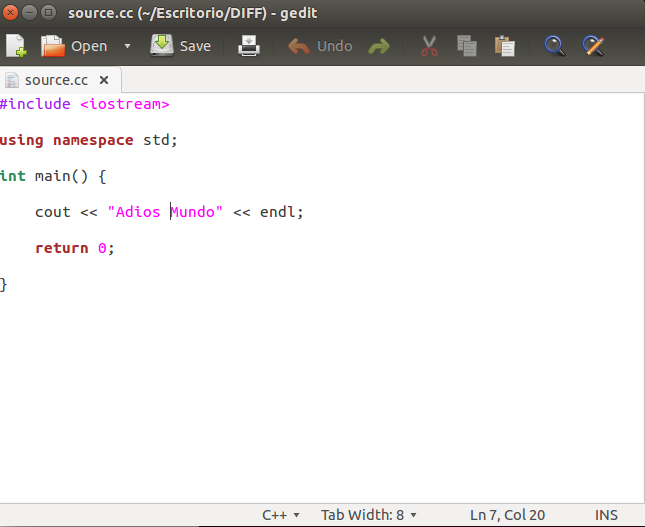
\includegraphics[scale=0.35]{pics/source.png}  
	\caption{source.cc} \label{fig:source.cc}
	\end{figure}

	\begin{figure}[H]
	\centering
	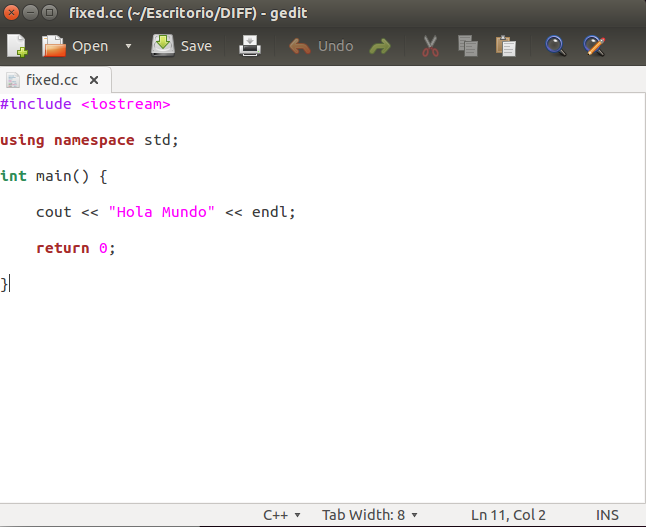
\includegraphics[scale=0.35]{pics/fixed.png}  
	\caption{fixed.cc} \label{fig:fixed.cc}
	\end{figure}

Para poder arreglarlo lo que haremos es obtener las diferencias entre ellos con \textit{diff source.cc fixed.cc} y lo guardamos en el fichero \textit{dif}, después simplemente le aplicamos con patch las modificaciones nuevas a source.cc con \textit{patch source.cc dif}, y por último decimos que si.

	\begin{figure}[H]
	\centering
	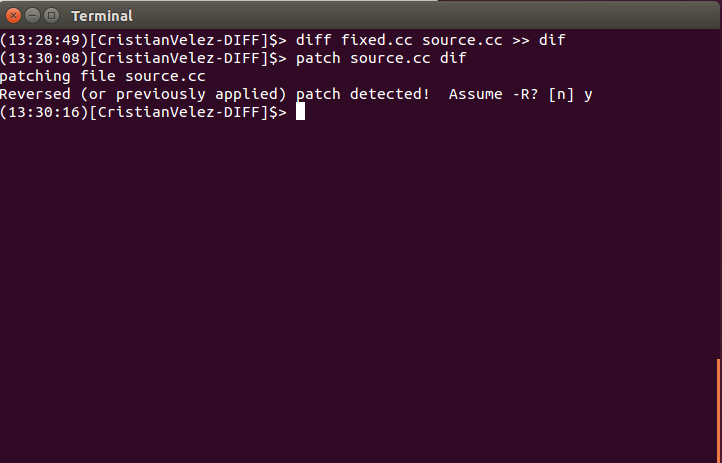
\includegraphics[scale=0.35]{pics/cambios.png}
	\caption{source.cc} \label{fig:sourcefixed.cc}
	\end{figure}

Ahora tenemos nuestro código parcheado,

	\begin{figure}[H]
	\centering
	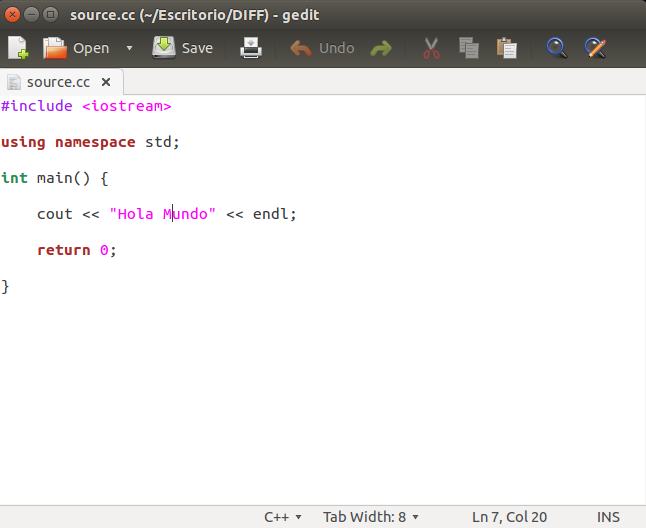
\includegraphics[scale=0.35]{pics/sourcefixed.png}
	\caption{sourcefixed.cc} \label{fig:sourcefixed.cc}
	\end{figure}


%----------------------------------------------------------------------------------------
%	Cuestión 12
%----------------------------------------------------------------------------------------
\section[Cuestión 12]{Realice la instalación de esta aplicación y pruebe a modificar algún parámetro de algún servicio. Muestre las capturas de pantalla	pertinentes así como el proceso de instalación.}

El proceso de instalación es muy sencillo, con ir a la documentación nos muestra un repositorio que podemos añadir y a continuación instalar.\cite{webmin}\\

\textit{cd /root}\\
\textit{wget http://www.webmin.com/jcameron-key.asc}\\
\textit{apt-key add jcameron-key.asc}\\
\textit{apt-get update}\\
\textit{apt-get install webmin}\\

Una vez realizado entramos en localhost:10000 y ponemos nuestro usuario y contraseña actual.

	\begin{figure}[H]
	\centering
	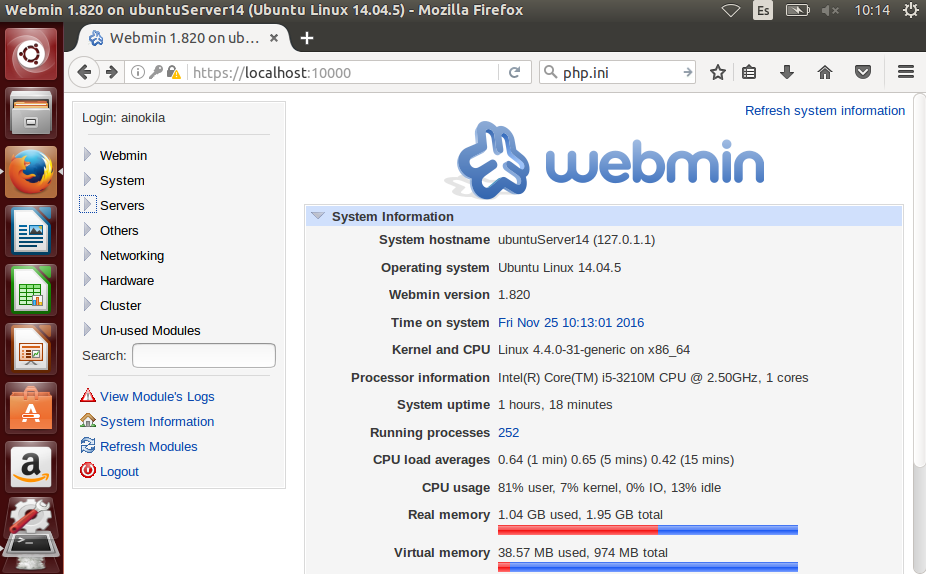
\includegraphics[scale=0.35]{pics/webmin1.png}
	\caption{Webmin} \label{fig:web_min}
	\end{figure}

Para la modificación voy a activar un script que habia desactivado en Cron,

	\begin{figure}[H]
	\centering
	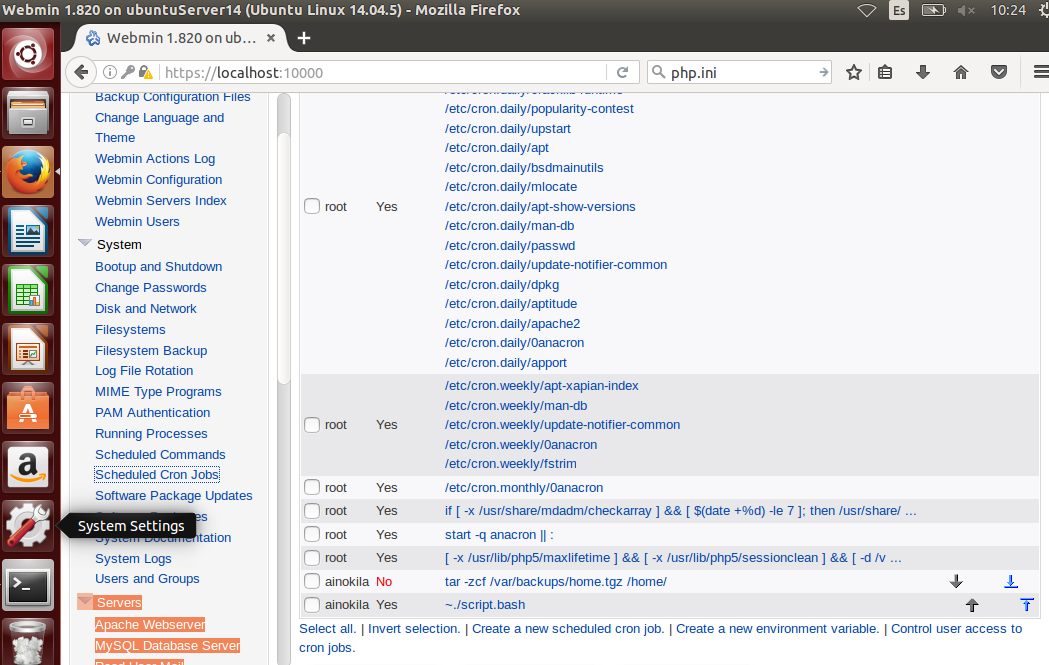
\includegraphics[scale=0.35]{pics/cron1.png}
	\caption{Webmin Cron 1} \label{fig:web_cron1}
	\end{figure}

Selecciono la tarea,

	\begin{figure}[H]
	\centering
	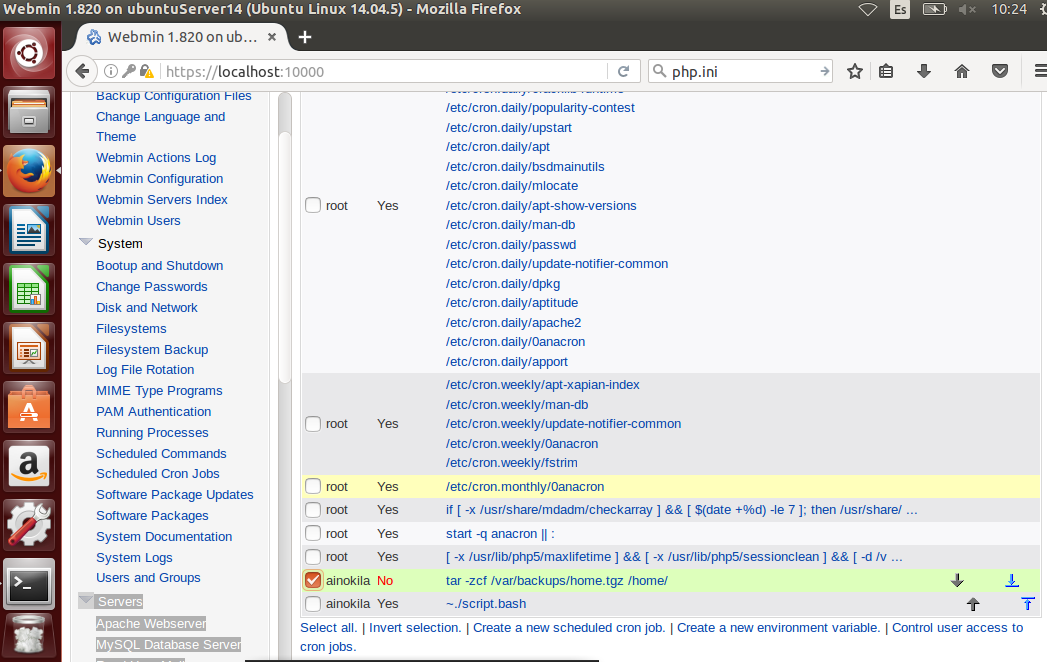
\includegraphics[scale=0.35]{pics/cron2.png}
	\caption{Webmin Cron 2} \label{fig:web_cron2}
\end{figure}

Doy a enable y finalmente ya esta activada la tarea,

	\begin{figure}[H]
	\centering
	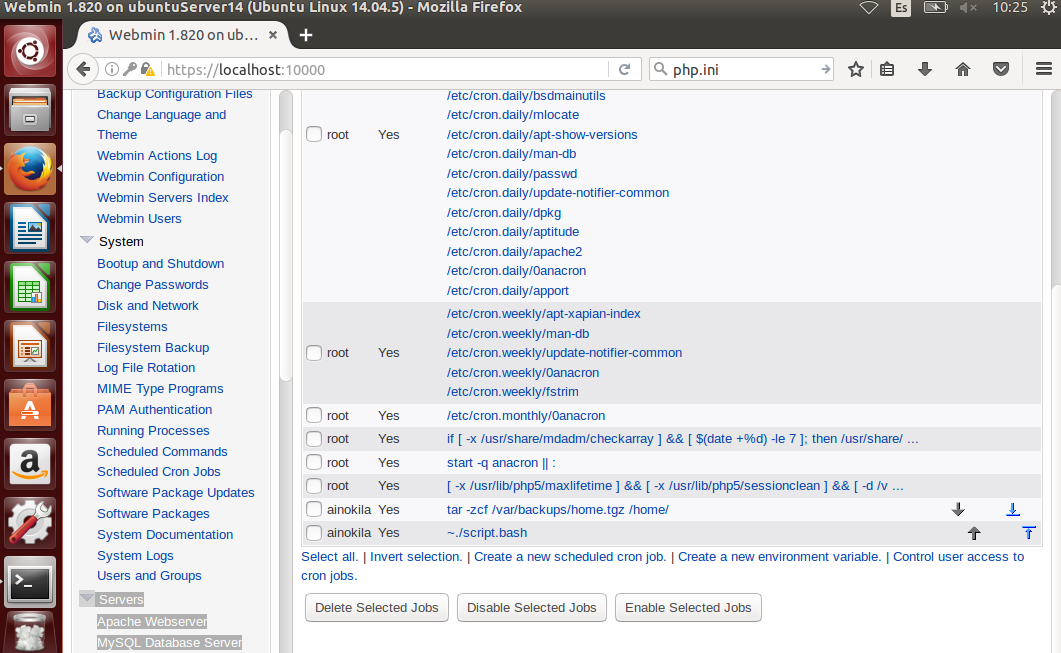
\includegraphics[scale=0.35]{pics/cron3.png}
	\caption{Webmin Cron 3} \label{fig:web_cron3}
	\end{figure}

%----------------------------------------------------------------------------------------
%	Cuestión 13
%----------------------------------------------------------------------------------------
\section[Cuestión 13]{Instale phpMyAdmin, indique cómo lo ha realizado y muestre algunas capturas de pantalla. Configure PHP para poder importar BDs de	hasta 25MiB (en vez de los 8 MiB de límite por defecto). Indique cómo ha realizado el proceso y muestre capturas de pantalla.}

Para instalar phpmyadmin, he lanzado el comando sudo apt-get install phpmyadmin, he puesto las contraseñas para las bases de datos y finalmente accedido con mi ip/phpmyadmin \cite{phpmyadmin}

	\begin{figure}[H]
	\centering
	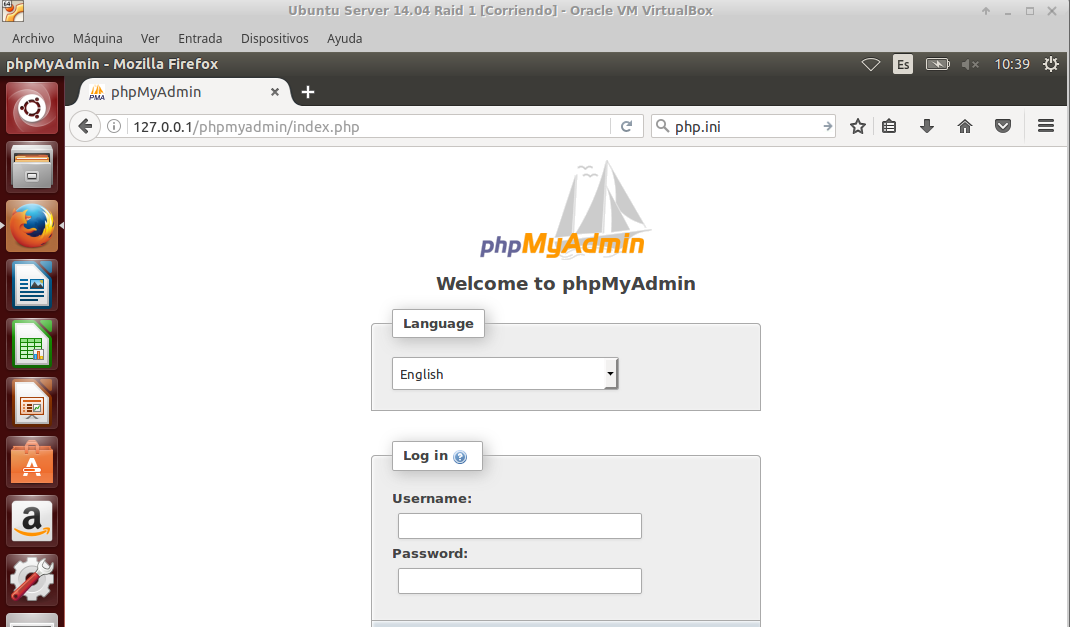
\includegraphics[scale=0.35]{pics/phpAdmin.png}
	\caption{Phpmyadmin} \label{fig:php_my_Admin}
	\end{figure}

Accedemos con root y la contraseña que pusimos anteriormente,

	\begin{figure}[H]
	\centering
	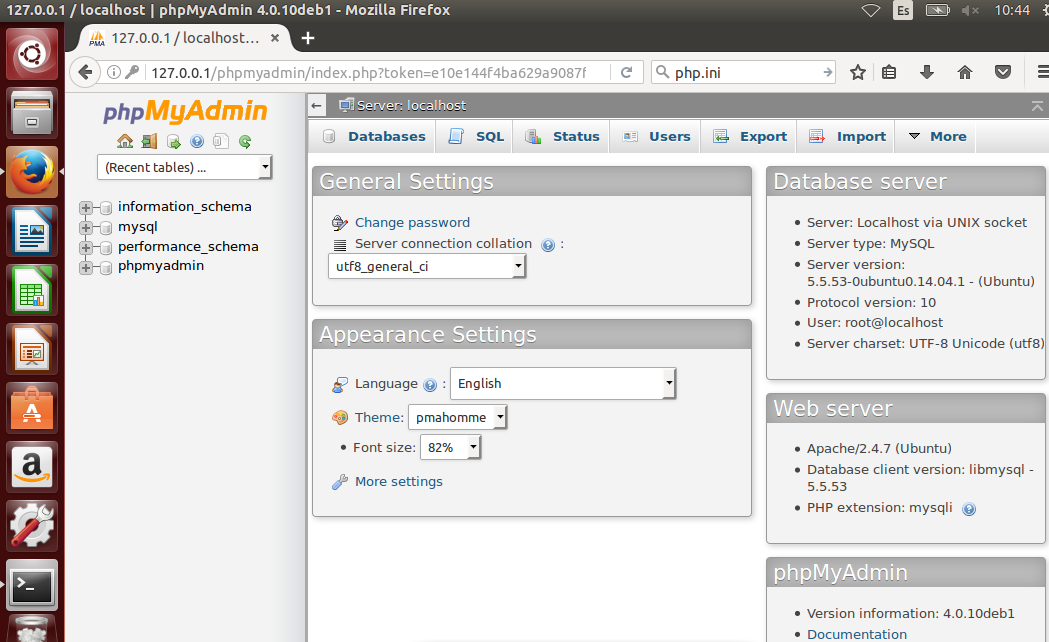
\includegraphics[scale=0.35]{pics/php_my2.png}
	\caption{Phpmyadmin 2} \label{fig:php_my_Admin2}
\end{figure}

Para poder subir ficheros mas grandes tenemos que modificar /etc/php5/apache2/php.ini y donde pone post\_max\_size cambiamos 8 por 25 y ya reiniciamos el servicio apache2.

	\begin{figure}[H]
	\centering
	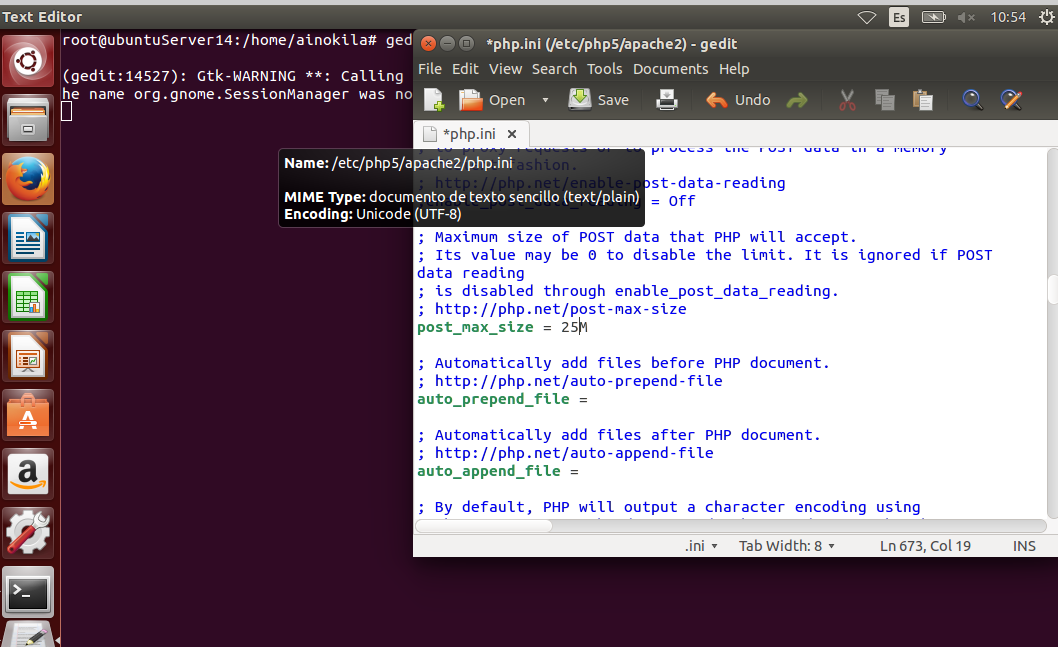
\includegraphics[scale=0.35]{pics/cambio_php.png}
	\caption{Subida 25 MiB} \label{fig:php_cambio}
\end{figure}


%----------------------------------------------------------------------------------------
%	Cuestión 14
%----------------------------------------------------------------------------------------
\section[Cuestión 14]{Visite al menos una de las webs de los software mencionados	y pruebe las demos que ofrecen realizando capturas de pantalla y	comentando qué está realizando.}

He probado la demo que ofrece IspConfig\cite{isp}

	\begin{figure}[H]
	\centering
	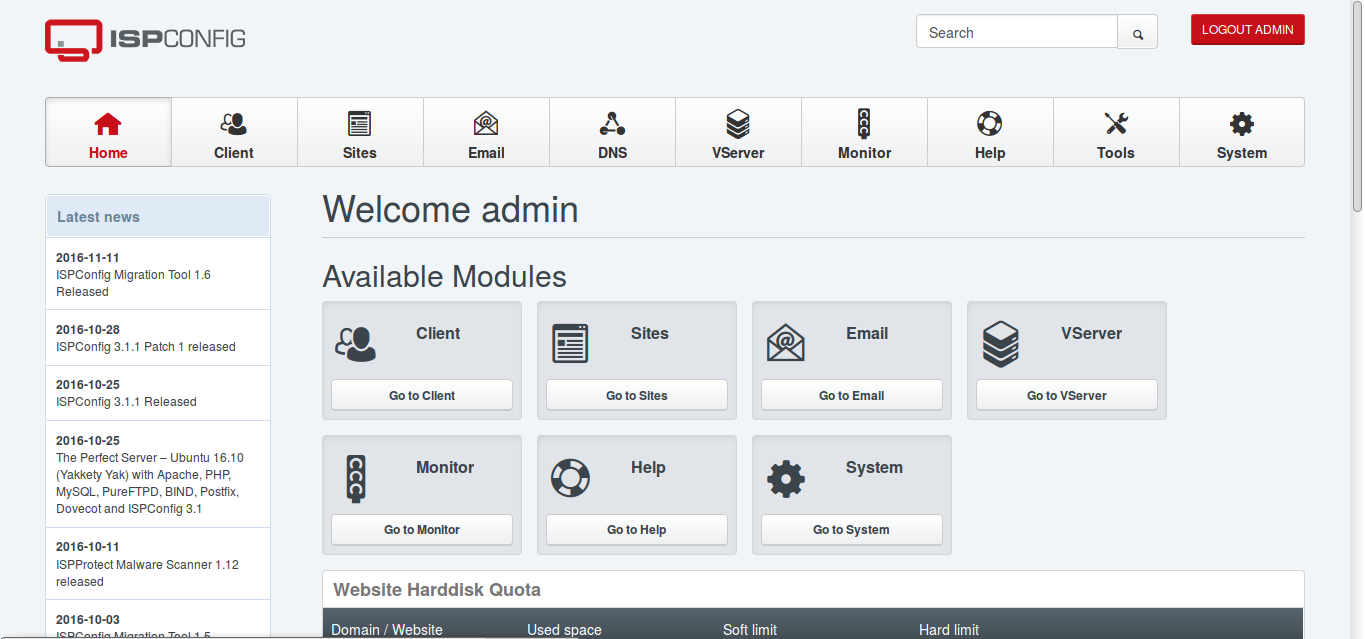
\includegraphics[scale=0.35]{pics/ejemplo_1.png}  
	\caption{IspConfig} \label{fig:isp_config1}
	\end{figure}

En esta opción podemos añadir nuevos clientes a Isp,

	\begin{figure}[H]
	\centering
	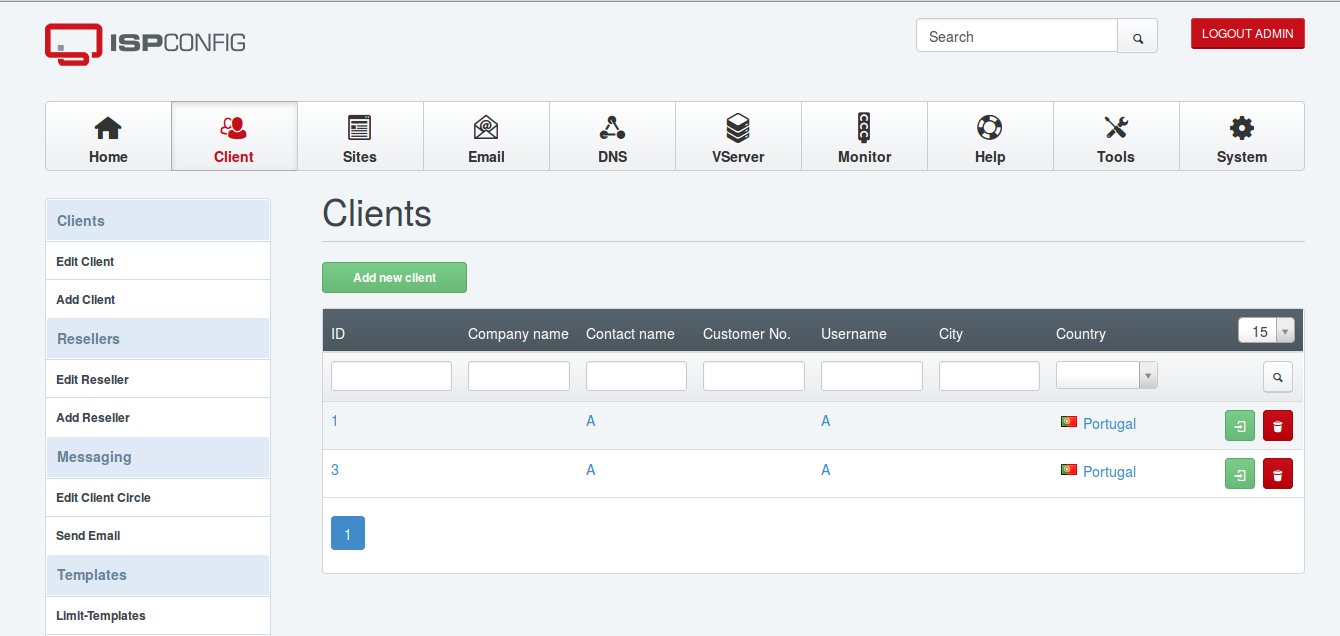
\includegraphics[scale=0.35]{pics/ejemplo_2.png}  
	\caption{IspConfig 2} \label{fig:isp_config2}
	\end{figure}

También ISP nos muestra opciones para modificar el correo, ver estado de los servidores y mas funciones.



%----------------------------------------------------------------------------------------
%	Cuestión 15
%----------------------------------------------------------------------------------------
\section[Cuestión 15]{a) Ejecute los ejemplos de find, grep b) Escriba el script que haga uso de sed para cambiar la configuración de ssh y reiniciar el servicio. c) Muestre un ejemplo de uso para awk}

\begin{enumerate}[label=(\alph*)]
	\item Ejecución:
		\begin{figure}[H]
		\centering
		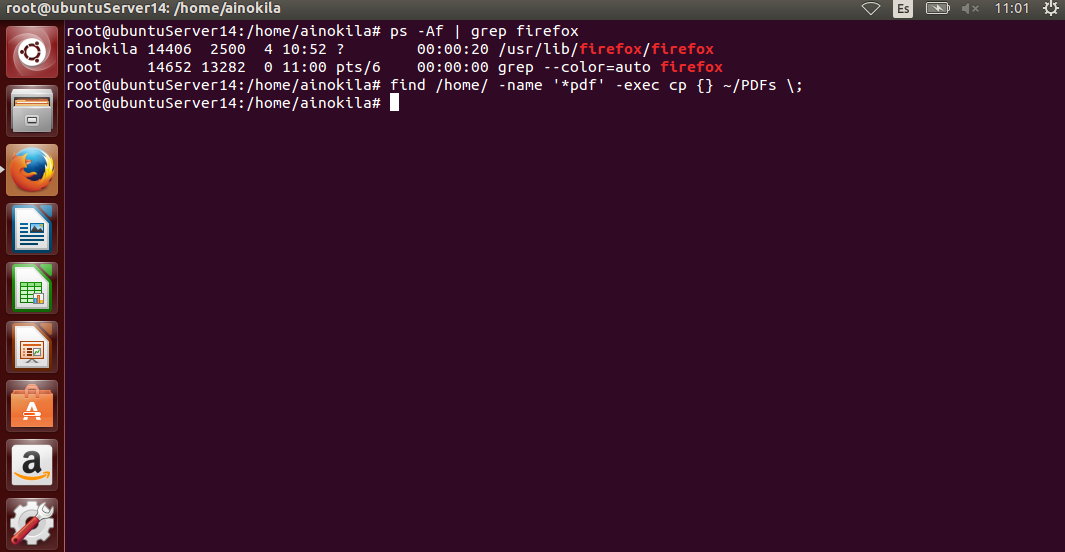
\includegraphics[scale=0.35]{pics/a.png}  
		\caption{Ejecución Comandos} \label{fig:ejecucion}
		\end{figure}
	
	\item Para poder cambiar el puerto 6666 de sshd basta con una expresión regular como  \textit{sed -i \'s\/\^Port .\*/Port 6666/g\' /etc/ssh/sshd\_config}
	
	\begin{figure}[H]
		\centering
		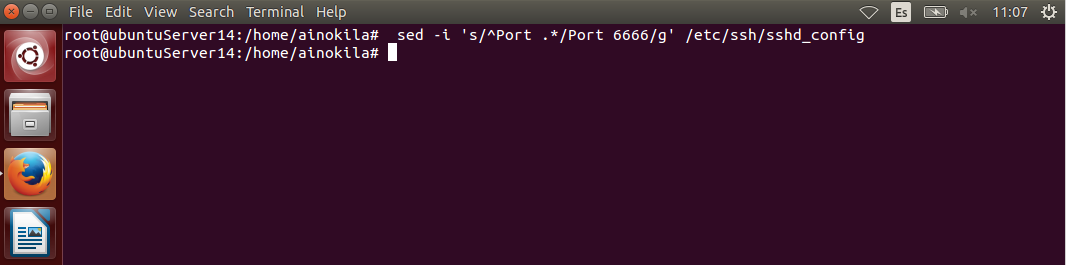
\includegraphics[scale=0.35]{pics/sed.png}  
		\caption{Cambio puerto} \label{fig:cambio_puerto}
	\end{figure}
	
	
	
\end{enumerate}
%----------------------------------------------------------------------------------------
%	Cuestión 16
%----------------------------------------------------------------------------------------
\section[Cuestión 16]{Escriba el script para cambiar el acceso a ssh usando PHP o Python.}

En Php junto a sed sería,

	\begin{figure}[H]
	\centering
	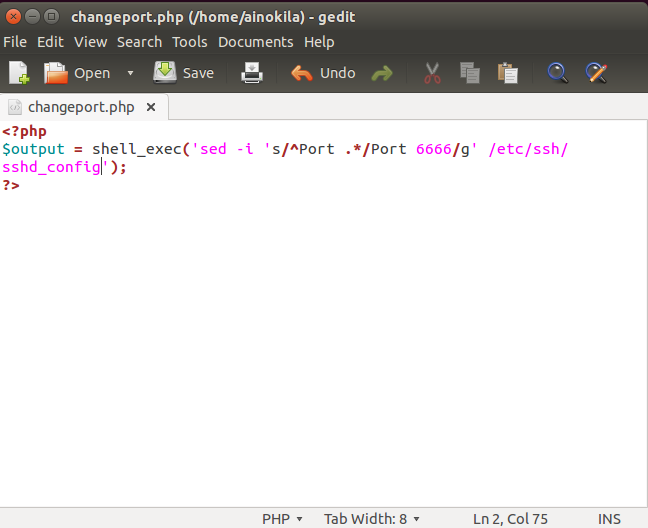
\includegraphics[scale=0.35]{pics/change_port_script.png}  
	\caption{Cambio puerto con PHP} \label{fig:cambio_puerto_PHP}
\end{figure}


%----------------------------------------------------------------------------------------
%	Cuestión 17
%----------------------------------------------------------------------------------------
\section[Cuestión 17]{Abra una consola de Powershell y pruebe a parar un programa en ejecución (p.ej), realice capturas de pantalla y comente lo que muestra.}

Para visualizar los procesos de powershell, usaremos el comando \textit{tasklist}\cite{tasklist} que nos mostrará los procesos,

	\begin{figure}[H]
	\centering
	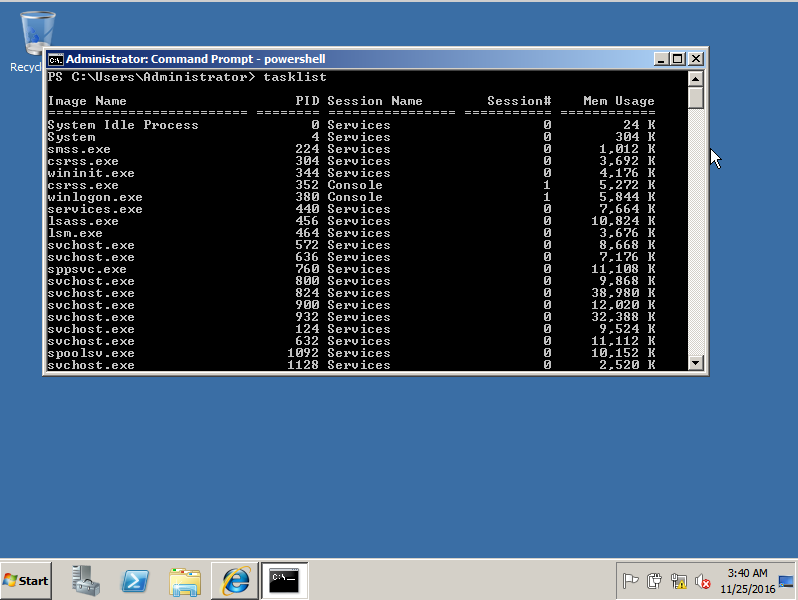
\includegraphics[scale=0.35]{pics/task.png}  
	\caption{Procesos} \label{fig:procesos}
	\end{figure}

Ahora vamos a parar un proceso, para ello usaremos \textit{stop-service <nombre>} \cite{micro},

	\begin{figure}[H]
	\centering
	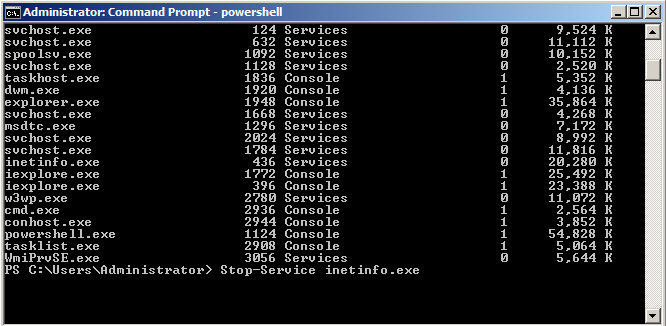
\includegraphics[scale=0.35]{pics/inet.png}  
	\caption{Parando proceso} \label{fig:inet}
\end{figure}


 




\bibliography{citas} %archivo citas.bib que contiene las entradas 
\bibliographystyle{plain} % hay varias formas de citar

\end{document}
\grid
